\documentclass[11pt]{article}

\usepackage{amsmath}
\usepackage{physics}
\usepackage{amssymb}
\usepackage{amsfonts}
\usepackage{hyperref}
\usepackage{thmbox}
\usepackage{geometry}
\usepackage{graphicx}

\newcommand{\R}{\mathbb{R}}
\newcommand{\C}{\mathbb{C}}
\newcommand{\Z}{\mathbb{Z}}

\newtheorem[L]{thm}{Theorem}[section]

\author{Haiyang Wang}
\date{\today}
\title{Fast Solver for 2D Stokes Flow}

\begin{document}

\maketitle

\begin{abstract}
  Plane Stokes flow models many problems in physics, biology and engineering. Here we exploit the \textit{return to Poiseuille} (see Section~\ref{sec:ret2poi}) to solve Stokes flow on complicated network of pipes, with the condition that the pipe network has enough straight components. 
\end{abstract}

\section{Introduction}

\subsection{Problem Description}

stokes 2d on a complicated pipe network. 

\begin{itemize}
  \item solving plane stokes equation on simple pipes.
  \item connecting the pipes to build a pipe networks. 
\end{itemize}

\subsection{Why does it matter}
todo. 
\subsection{Related works}
todo.

\paragraph{hemholtz eq, the normal mode analysis}

\paragraph{stokes eq, similar complex networks}

\subsection{What I have done}



\subsection{This paper is organized as following}

\section{Math Preliminaries}

It is well-known that plane Stokes equation is closely related to the biharmonic equation. In this section, we transform the Stokes boundary value problem (\ref{stokes}-\ref{bdr-velocity}) into a biharmonic boundary value problem (\ref{stream-2},\ref{stream-bv}). Then, Goursat's formulae and Sherman-Lauricella representation will give a boundary integral equation, which will be solved numerically. 

The previous paragraph is no more than what's done in (cite professor greengard's paper). The new idea in this paper is to exploit the \textbf{return to Poiseuille} phenomenon: Stokes flow in a straight pipe will converge to the Poiseuille flow in the axial direction at an exponential rate. This is proved analytically in (cite some paper proving this, using a figure as an example). As in (some figure), return to Poiseuille allow us to assume the flow is almost Poiseuille away from irregular (not straight pipe) area. 

Therefore we can break the domain, at where the flow is almost Poiseuille, into subdomains. And we can assume that the subdomains have the boundary value of a Poiseuille velocity profile. Then, we can solve the Stokes equation for each sub-domain and then glue the solutions of each subdomain to get a very accurate solution for the global domain. 

Other way around, we can build the solvers for some standard shapes of pipes. Connecting these pipes can give us a very complicated network of pipes. And we can solve the Stokes equation on this pipe network by simply matching the local solvers at the boundary. This saves much time compared to solving the Stokes equation directly. 


\subsection{Stokes Boundary Value Problem}

The plane linear Stokes equation is
\begin{align}
  \nu \Delta u = \frac 1 \rho \pdv{p}{x},\quad &\nu \Delta v = \frac 1\rho \pdv{p}{y} 
  \label{stokes} \\
  u_x + v_y &= 0
  \label{continuity}
\end{align}
where $u,v$ are components of velocity, $\rho$ is the density, $\nu$ is the viscosity, and $p$ is the pressure. Additionally, vorticity is defined as $\zeta  = u_y - v_x$. It is easy to see that vorticity is harmonic because of (\ref{stokes}):
\begin{align}
  \Delta \zeta = \Delta u_y - \Delta v_x = \frac 1{\nu \rho} p_{xy} -  \frac 1{\nu \rho} p_{xy} =0 \label{vorticity-harmonic}
\end{align}

We are interested in the boundary value problems on a finite domain $D\subset \mathbb R^2$, with the the $(M+1)$-ply connected boundary $\partial D =  \Gamma = \Gamma_0 \cup \Gamma_1 \cup \cdots \cup \Gamma_M$ is , where $\Gamma_0$ is the outer boundary of $D$, and $\Gamma_1,\cdots, \Gamma_M$ are the interior contours of $D$. The boundary value of our interest is velocities on the boundary: 
\begin{align}
  u = h_2(t),\quad v = - h_1(t), \quad t\in \Gamma
  \label{bdr-velocity}
\end{align}

(insert a picture here of an example domain.)


\subsection{The Biharmonic Boundary Value Problem}


$(\ref{continuity})$ is equivalent to the existence of the stream function $W(x,y)$ such that:
\begin{align}
  W_x = -v, \quad W_y = u \label{stream-1}
\end{align}
($\ref{vorticity-harmonic}$) indicates that stream function satisfies the biharmonic equation:
\begin{align}
  \Delta^2 W(x,y) 
  &= \Delta (W_{xx} + W_{yy}) = \Delta (-v_{x} + u_{y}) = \Delta \zeta = 0 
  \label{stream-2}
\end{align}
And the velocity boundary condition ($\ref{bdr-velocity}$) can be understood as the boundary conditions :
\begin{align}
  W_x(t) = h_1(t), \quad W_y(t) = h_2(t), \quad t\in \Gamma
  \label{stream-bv}
\end{align}

\subsection{Goursat's Formulae}

Any plane biharmonic function $W(x,y)$ can be expressed by Goursat's formulae as 
\begin{align}
  W(x,y) = \Re (\bar z \phi(z) + \chi (z)) \label{Goursat}
\end{align}
where $\phi, \chi$ are analytic functions of complex variable $z = x+yi$. 

Simple calculations lead to the following useful formulae:
\begin{align}
    u(x,y) + iv(x,y) 
    &= \phi(z) + z \overline{\phi'(z)} + \overline{\psi(z)}
    \label{g-velocity}\\
  \zeta(x,y) + \frac i\nu p(x,y) &= 4\phi'(z) \label{g-vorticity}
\end{align} where $\psi = \chi'$. 

\eqref{g-velocity} transforms the boundary condition \eqref{stream-bv} to 
\begin{align}
  \phi(t) + t\overline{\phi'(t)} + \overline{\psi(t)} 
  = h(t), \quad
  t \in \Gamma
\end{align} where $h(t) =  h_1(t) + ih_2(t)$. $t$ need to be understood as a complex number in the LHS and a plane coordinate in the RHS. This is a slight \textbf{abuse of notation} that will not be explained later. 

\subsection{Sherman-Lauricella Representation}

(citing professor Greengard's paper) suggested the following Sherman-Lauricella integral representation: 

\begin{align}
  \phi(z) &=
    \frac {1}{2\pi i} \int_\Gamma \frac{\omega(\xi)}{\xi - z} d\xi  
    + \sum_{k=1}^M C_k \log (z-z_k)
    \\
  \psi(z) &=
    \frac {1}{2\pi i} \int_\Gamma \frac{\overline{\omega(\xi)}d\xi +  \omega(\xi)\overline{d\xi}}{\xi - z}  
    - \frac {1}{2\pi i} \int_\Gamma \frac{\overline{\xi} \omega(\xi)}{(\xi - z)^2} d\xi  
    \\
    & \quad + \sum _{k=1}^M \frac{b_k}{z-z_k}  
      + \sum_{k=1}^M \overline C_k \log (z-z_k) - \sum_{k=1}^M C_k \frac{\overline z_k}{z-z_k} \nonumber
\end{align}
where $\omega$ is an unknown complex density on $\Gamma$, $z_k$ is an arbitrarily prescribed point inside the component curves $\Gamma_k$, and $$C_k = \int_{\Gamma_k} \omega(\xi) |d\xi|$$
It is important to obeserve that $\phi,\psi$ might be multiply-valued functions, but velocity, pressure, and vorticity should be single-valued functions. 


Letting a point $z$ in the interior of $D$ approach to a point on the boundary $\Gamma$, the classical formulae for the limiting values of Cauchy-type integral gives us the an integral equation for $\omega$:
\begin{align}
  \omega(t) 
  &+ \frac 1{2\pi i} \int_{\Gamma} \omega(\xi) d \ln \frac{\xi - t}{\overline{\xi - t}} - \frac 1{2\pi i} \int_\Gamma \overline{\omega(\xi)} d \ln \frac{\xi - t}{\overline{\xi - t}} \\
  &+ \frac{\overline b_0}{\bar t - \bar z^*} + \sum_{k=1}^M \frac{\bar b_k}{\bar t- \bar z_k} + \sum_{k=1}^M 2C_k \log |t-z_k| + \sum_{i=1}^M \bar C_k \frac{t-z_k}{\bar t - \bar z_k} \\
  =& h(t)
\end{align}
where $b_0$ vanishes on the natural compatibility condition $\Re \int_\Gamma \bar h(t) dt = 0$, which means there is zero net flux across $\Gamma$. The invertibility of the integral equation should follow from (citing some paper).\footnote{or should I try to prove it by myself? That would be a good practice on understanding the invertibility of integral equations. And I don't really understand them...} 

\subsection{Return to Poiseuille} 
\label{sec:ret2poi}

Return to Poiseuille is formulated on the domain of a semi-infinite pipe $D_L = \{(x,y)\mid x \ge 0, |y| \le L\}$, with the boundaries 
\begin{align}
  \Gamma_L &=&& \Gamma_L^1\quad\quad\quad& \cup &\Gamma_L^2 &\cup&\Gamma_L^3 \\
  &=&&\{(0,y)||y| \le L \}& \cup &\{(x,L)|x\ge 0\} &\cup& \{(x,-L)\mid x\ge 0\}\nonumber
\end{align}
where $\Gamma_L^1$ is the inflow, $\Gamma_L^2,\Gamma_L^3$ are walls, which means they have the non-slippery boundary conditions. So, the boundary conditions on $\Gamma_L$ is of the following form: 
\begin{align}
  &W_x(0,y) + iW_y(0,y) &&= -v(0,y) + iu(0,y),& \quad |y|\le L\\
  &W_x(x,\pm L) + iW_y(x,\pm L) &&= 0,& \quad x\ge 0
\end{align}
where $u,v$ are velocities given at the boundary. Therefore the flux at the inflow $x=0$ is $F = \int -u(0,y) dy$. 

The Poiseuille velocity profile on this domain with flux $F$ is 
\begin{align}
  u_{poi}(x,y) &= \frac{4F}{3L^3} L^2 - y^2,\\
  v_{poi}(x,y) &= 0 
\end{align}
where the subscript $poi$ stands for Poiseuille. 

We want to prove that the difference 
\begin{align}
  \begin{pmatrix}
    \tilde u\\
    \tilde v
  \end{pmatrix} = 
  \begin{pmatrix}
    u\\v
  \end{pmatrix} - 
  \begin{pmatrix}
    u_{poi}\\v_{poi}
  \end{pmatrix}
\end{align}
decays exponentially as $x\to \infty$. Since all PDE in this paper is homogeneous and linear, $\bar u, \bar v$ can be solved through the biharmonic equation for $\tilde W = W - W_{poi}$:
\begin{align}
  \Delta \tilde W(x,y) &= 0, 
    &(x,y) \in D_L \label{ret2poi1} \\
  \tilde W_x(0,y)  &=  -v(0,y), 
     &|y| \le L \label{zero-flux-bc1}\\
  \tilde W_y(0,y)  &= u(0,y) - u_{poi}(0,y), 
     &|y| \le L \label{zero-flux-bc2}\\
  \tilde W_x(x,\pm L)  &= 0,\quad  \tilde W_y(x,\pm L) = 0, &x\ge 0 \label{zero-flux-bc3}
\end{align}

Without lost of generality, assuming that $\tilde W(0,-1) = 0$. Then
 boundary conditions \eqref{zero-flux-bc1},\eqref{zero-flux-bc2}, and \eqref{zero-flux-bc3} can be rewritten as:
 \begin{align}
    \tilde W(x,\pm L) = 0, \quad &&
      \pdv{\tilde W}{\nu} (x,\pm L) = 0, \quad  &&
      x\ge 0 &&\\
    \tilde W(0,y) = \int_{-L}^y \tilde{W}_y(0,\eta)d\eta, \quad &&
      \pdv{\tilde W}{\nu} (0,y) = v(0,y), \quad &&
      |y|\le L \label{ret2poi-1}
 \end{align}where $\pdv \nu$ denotes the out normal derivative. 

For return to Poiseuille phenomenon, one should expect that 
\begin{align}
  A(x) = \sqrt{\int_{-L}^L\tilde u^2(x,y)+\tilde v(x,y)^2 dy} \le A\exp(-kx)
\end{align} 
where $A$ depends on $L, u(0,y), v(0,y)$, and $k$ depends only on $L$. [Horgan 1989] has summarized the result on $k$:
\begin{itemize}
  \item $k = \frac{4.2}{2L}$. \footnote{this is the smallest real part of the roots of $\sin z + z = 0, \Re z > 0$} This is the predicted value given by the analysis of Papkovich-Fadle eigenfunctions, which is complete basis for the problem (\ref{ret2poi1}-\ref{ret2poi-1}) given that $u(0,y),v(0,y)$ and their first few derivative has bounded-variation. See Gregory 1980 for this result. However, this is not proven yet to the best of author's knowledge. 
  \item $k= \frac{2.7}{2L}$. Although this value is smaller than the previous one. It has been proven in Knowles 1983. This is the best value of $k$ that I know of. 
\end{itemize}


\paragraph{Remark} Pretending that $k=\frac{4.2}{2L}$ gives a valid bound. Then, if the pipe has the length of $10L$, the flow should be Poiseuille at the outlet, up to an error of order of machine precision, regardless of the flow at the inlet. \footnote{I should spell out the regularity conditions along with the equations} In real situations, the difference to Poiseuille converges to $10^{-13}$, the numerical error of my Nyestorm discretization, at $7.5L$. So this return to poiseuille approximation really makes sense. 

\subsubsection{plotting the estimate against the true error}
todo. 

\subsection{perhaps also some potential theory}

hmmm, I don't know that to write in this section. 

\subsection{Summary}

In this section, we have articulated the integral equation for Stokes flow in terms of the stream function $W$.  And we have supplied the reasons why \textbf{return to Poiseuille} is a reasonable assumption to make. 

Given the above, we can do the following 

\begin{itemize}
  \item For each pipe, with the inlets and outlets being sufficiently long, $\ge 7.5 L$ as suggested by numerical experiment, straight pipe, we can build a solver of this pipe with Poiseuille boundary conditions. 
  \item We can connect these pipes and their solvers on their inlets and outlets, based on the restriction of flux and single-valuedness of the pressure function. 
  \item Connecting the solvers of thes pipes will give us a solver for a network of pipes, which could be rather complicated and takes days for a direct solution. 
\end{itemize}


\newpage
\section{Numerical Algorithms}

\subsection{discretizing the geometry}

\subsection{Integral equation}

\subsection{Smoothed Corners}
\begin{figure}[hbt]
  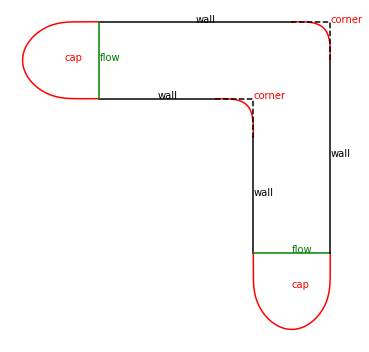
\includegraphics[width=10cm,height=10cm,keepaspectratio]{pic/smooth.png}
  \caption{Smoothed corners}
  \label{smoothed-corner}
\end{figure}


Initially, the geometry of our consideration has corners that would not work well with the Nyst\"orm discretization scheme. For this reason we have smoothed all corners. This gives us spectral convergence of the Nyst\"orm discretization. See 

Figure~\ref{smoothed-corner} demonstrates how the corners that smoothed. The original geometry is a 90 degree band, which has the walls (black line) and flows (green line). 
\begin{itemize}
  \item The 1st type of corners (dashed black line) are part of the walls, they are replaced by the smooth red lines. See [O'Neil 2016] for construction of the smooth red line. 
  \item The 2nd type of corners are around the flow (green line), and they are replaced with the red caps. As explained in Section~\ref{sec:ret2poi}, velocity profile at the inlet/outlet is assumed to be Poiseuille up to a negligible error. This assumption means that velocity profile at the flows (green lines) and the caps (red lines) should both be Poiseuille. Therefore, when building the solver, we replace the green line with the red cap with the same boundary Poiseuille velocity profile. When connecting tubes, we still connect them along the green lines. This would introduce a small error that is bounded by the negligible error of "return to Poiseuille" hypothesis. The caps are constructed according to [Bagge 2021]. 
\end{itemize}


\subsection{how to combine local solvers}

\section{numerical results}

\subsection{plot the analytic error bound in assuming return to poiseuille}
\subsection{plot the numerical error for such assumptions}
\subsection{plotting the error of combining local to global}
\subsection{solve for a complicated network of pipes to show the power of this method}

\section{Conclusions}
\subsection{summarize what I've done}
\subsection{outlook. What other work might be followed?}

\end{document}

